\documentclass{article}
\usepackage{listings}             % Include the listings-package
\usepackage[usenames,dvipsnames,svgnames,table]{xcolor}
\usepackage{graphicx}
\usepackage{hyperref}
\usepackage{amsmath}
\usepackage{csquotes}
\usepackage{changelog}

\definecolor{mygreen}{rgb}{0,0.6,0}
\definecolor{mygray}{rgb}{0.5,0.5,0.5}
\definecolor{mymauve}{rgb}{0.58,0,0.82}

\newcommand{\SmartVersion}{1C}
    
\title{SmartCTF}
\author{The\_Cowboy}
\pagestyle{headings}
\begin{document}
\maketitle
\lstset{language=Java}          % Set your language (you can change the language for each code-block optionally)
\section{Introduction}

\lstset{ %
  backgroundcolor=\color{white},   % choose the background color; you must add \usepackage{color} or    %\usepackage{xcolor}
  basicstyle=\footnotesize,        % the size of the fonts that are used for the code
  breakatwhitespace=false,         % sets if automatic breaks should only happen at whitespace
  breaklines=true,                 % sets automatic line breaking
  captionpos=b,                    % sets the caption-position to bottom
  commentstyle=\color{mygreen},    % comment style
  deletekeywords={...},            % if you want to delete keywords from the given language
  escapeinside={\%*}{*)},          % if you want to add LaTeX within your code
  extendedchars=true,              % lets you use non-ASCII characters; for 8-bits encodings only, %does not work with UTF-8
  frame=single,                    % adds a frame around the code
  keepspaces=true,                 % keeps spaces in text, useful for keeping indentation of code %(possibly needs columns=flexible)
  keywordstyle=\color{blue},       % keyword style
  language=Java,                 % the language of the code
  morekeywords={*,...},            % if you want to add more keywords to the set
  numbers=left,                    % where to put the line-numbers; possible values are (none, left, %right)
  numbersep=5pt,                   % how far the line-numbers are from the code
  numberstyle=\tiny\color{mygray}, % the style that is used for the line-numbers
  rulecolor=\color{black},         % if not set, the frame-color may be changed on line-breaks within %not-black text (e.g. comments (green here))
  showspaces=false,                % show spaces everywhere adding particular underscores; it %overrides 'showstringspaces'
  showstringspaces=false,          % underline spaces within strings only
  showtabs=false,                  % show tabs within strings adding particular underscores
  stepnumber=2,                    % the step between two line-numbers. If it's 1, each line will be %numbered
  stringstyle=\color{mymauve},     % string literal style
  tabsize=2,                       % sets default tabsize to 2 spaces
  title=\lstname                   % show the filename of files included with \lstinputlisting; also %try caption instead of title
} %optionally)

SmartCTF is a Mutator/ServerActor which reinforces and encourages the collaborative ``Teamplay'' by rewarding the players ``Smartly''.  Furthermore, the aim is to display the complete information required for a decent ``Multiplayer'' team game which includes TickRate, Current/Elapsed game time and ``Collective Ping/Netspeed'' of the teams.

\begin{figure}
\centering
\label{fig:smartscoreboard}
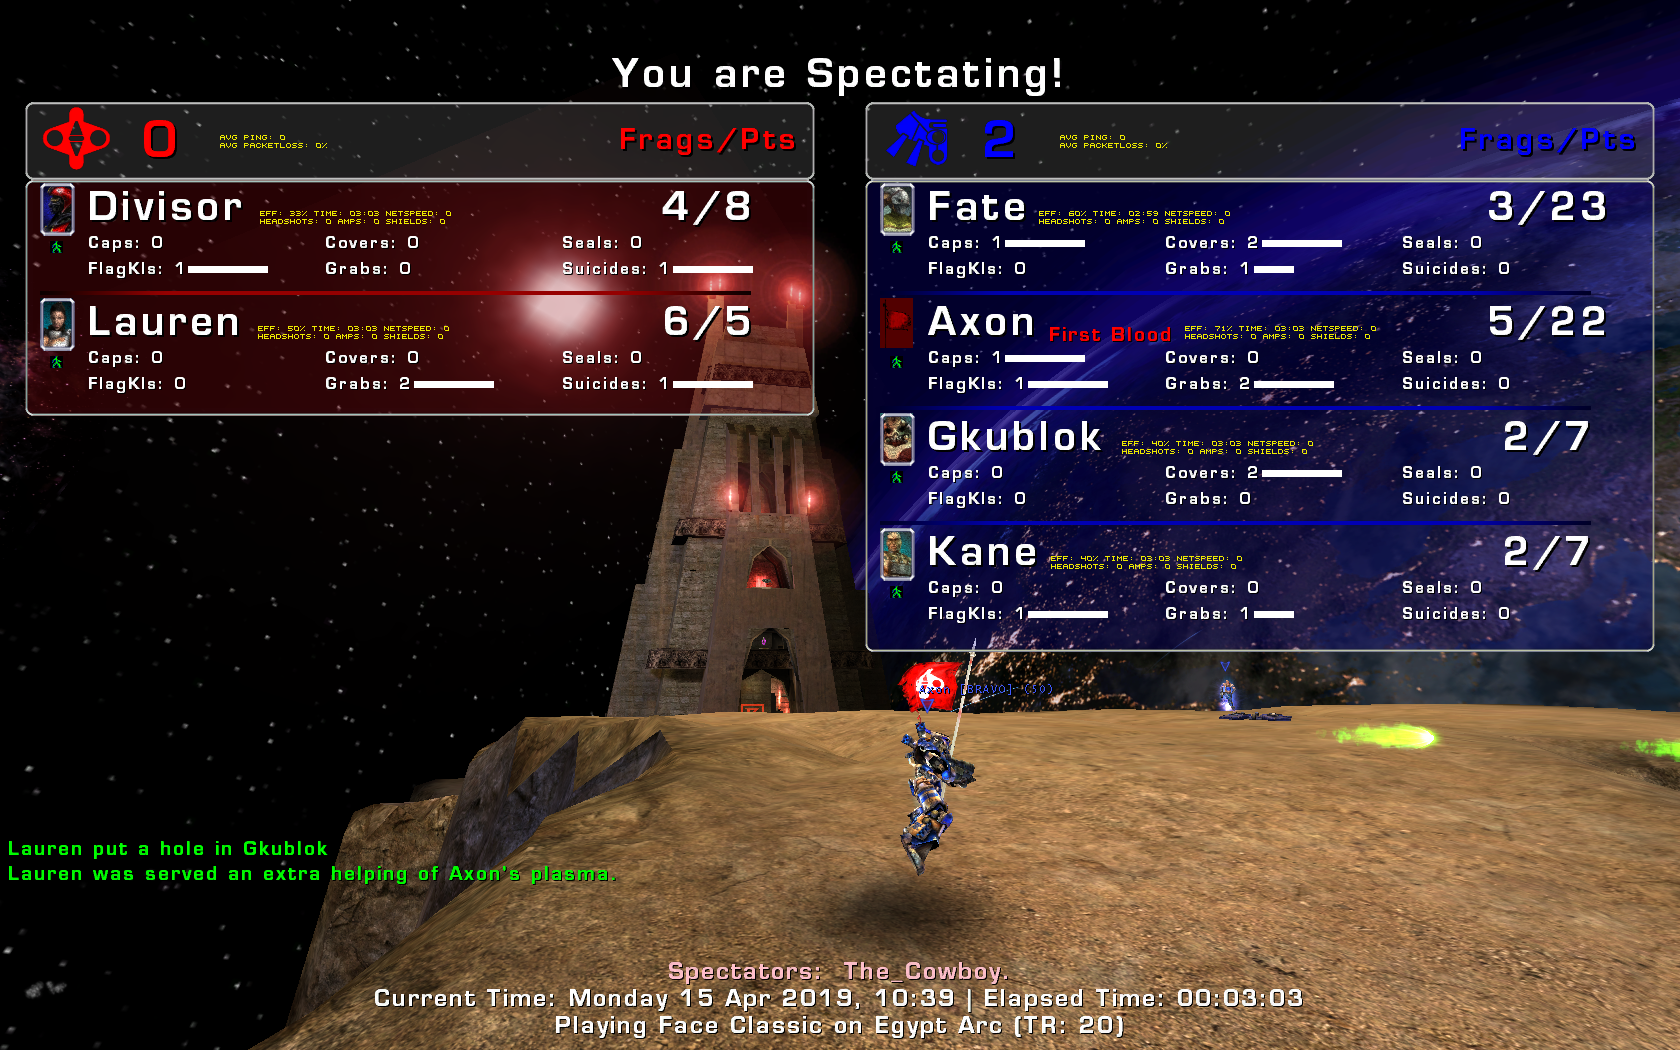
\includegraphics[width=1.1\textwidth]{img}
\caption{A screenshot of the SmartCTF\SmartVersion~Scoreboard.}
\end{figure}

SmarCTF (for \href{https://en.wikipedia.org/wiki/Unreal_Tournament}{\color{Blue}UnrealTournament}) has been developed for over a decade by several ``Coder Players'' to meet the dynamic needs of the manifold of modern ``PlayerBase''.  For the accurate chronological timeline click \href{http://wiki.unrealadmin.org/SmartCTF}{{\color{Blue}here}}.

This document concerns with the incarnation of SmartCTF (version \SmartVersion) for \href{https://en.wikipedia.org/wiki/Unreal_Tournament_2004}{{\color{Blue}UT2004}}. 

\section{Installation}

\begin{itemize}
\item place the {\color{Orange}SmartCTF\SmartVersion.u} and {\color{Orange}SmartCTF\SmartVersion.ucl} files in the {\ttfamily System} directory.
\item place the {\color{Orange}CountryFlags2.utx} in the {\ttfamily Textures} directory.  For Client install, you are done.  Load the SmartCTF\SmartVersion~ from mutator list in the game.
\item for Server install, in the {\color{Purple}UT2004.ini} or {\color{Purple}Server.ini}, add the line\\

  \fbox{%
    \parbox{\textwidth}{%
        ServerPackages = SmartCTF\SmartVersion\\
        ServerPackages = CountryFlags2
    }%
}\\

Note: SmartCTF\SmartVersion~ should be loaded as a mutator via appropriate command line\\

   \fbox{%
    \parbox{\textwidth}{%
        ?mutator=SmartCTF\SmartVersion.SmartCTF
    }%
}
\\

Furthermore, admin needs to set the ``Red(Blue)FlagZone'' for each CTF map individially (via Mapvote, see Section \ref{sec:configuration}).\item If you don't ``trust'' the SmartCTF's default QueryServerHosts (located in IpToNation.ini) you can upload the scripts in {\ttfamily MasterServerv1.6} on the PHP webserver as per the readme there.  The original PHP scripts should work so I haven't renamed/ported them. 
\end{itemize} 

\section{Configuration}
\label{sec:configuration}
There are three configurable sections of settings for SmartCTF\SmartVersion.  All these categories can be found in the {\color{Purple}UT2004.ini} or {\color{Purple}Server.ini}\footnote{Since version 1C, all configurable settings are stored in single ini.}.
\subsection{SmartCTF}
\label{subsec:smartctf}
The {\color{Orange}SmartCTF.ini} file is included with the package and contains the following section\\

 \fbox{%
    \parbox{\textwidth}{%
        [SmartCTF\SmartVersion.SmartCTF]\\
        bShowLogo=True\\
        CoverReward=2\\
        CoverAdrenalineUnits=5\\
        SealAward=2\\
        SealAdrenalineUnits=5\\
        RedFlagZone=RED BASE LOWER LEVEL\\
        BlueFlagZone=BLUE BASE LOWER LEVEL\\
        ScoreBoardType=SmartCTF\SmartVersion.SmartCTFScoreBoard\\
        bShowFCLocation=True\\
        bBroadcastMonsterKillAndAbove=True\\
        bDisableOvertime=False\\
        bShowCountryFlags=True\\
        bShowFirstBlood=True\\
        bRecoverTotalScore=True
    }%
} \\

Most configurable variables are self-explanatory. To identify a ``Seal'', the admin must recognize the mapzones with the flags.  In order to do that, start the game with the CTF map and stand near the flag.  Then give some order (``Defend the Flag" etc) which will reveal the zone you are standing in.  For example in CTF-FaceClassic, the RedFlagZone is ``RED BASE LOWER LEVEL'' and so on.  Different maps may have different Flag zone names (if the author has been decent enough to define zones).

bShowFCLocation if set true will display the team FC location at the top of the HUD to all the team players.

bBroadcastMonsterKillAndAbove if set to true will broaccast the Monsterkill message to all the players when someone achieves it.

bDisableOvertime if set to true will disable the default overtime and end the game in draw if both the teams have same score.  This feature was implemented on the request made \href{https://miasma.rocks/index.php?topic=1357.msg19336#msg19336}{\color{Blue}here}.

bShowCountryFlags will hide the country flags of the players when set to false.  bShowFirstBlood will hide the ``{\color{Red}First Blood}'' indicator on the scoreboard if set to false.

bRecoverTotalScore if set to true will recover the total player score when they rejoin the server.  Make sure there are no stats recovery mutators present when set to true.  Note: smart statistics are always restored irrespective of this option being true or false.

\subsection{IpToNation.ini}
SmartCTF has built in IpToNation mutator which is based on IpToCountry mutator developed by [es]Rush and Matthew 'MSuLL' Sullivan for UT99.  An excerpt from the IpToCountry readme

\begin{displayquote}
 ``To your knowledge, resolving a country from an IP requires quite a big database and implementing
it in UnrealScript would be very hard, thus IpToCountry connects to a PHP script which is located
on a web server. This PHP script uses a database kindly distributed by www.maxmind.com
If you want to know how the querying stuff exactly works just "Use the source Luke!"

AOL is quite troublesome. AOL has all its IP ranges registered in the USA and thus it doesn't
make identification easy. Fortunately Rush found a way to go around the problem.
Three major countries where AOL is very popular are: USA, Great Britain and Germany. All those three have
different timezones, so Rush just had to get a player's time and compare it to GMT. The idea maybe was Rush's
but Cratos was the first to implement it in LeagueAS, Rush got some code from him so big thanks, mate.''
\end{displayquote}

Now to configure, open {\color{Purple}UT2004.ini} or {\color{Purple}Server.ini} and browse to section\\
\fbox{%
    \parbox{\textwidth}{%
        [SmartCTF\SmartVersion.LinkActor]\\
        QueryServerHost[0]=iptocountry.ut-files.com\\
        QueryServerHost[1]=www.ut-slv.com\\
        QueryServerHost[2]=utgl.unrealadmin.org\\
        QueryServerHost[3]=\\
        QueryServerFilePath[0]=/iptocountry16.php\\
        QueryServerFilePath[1]=/iptocountry/iptocountry16.php\\
        QueryServerFilePath[2]=/iptocountry16.php\\
        QueryServerFilePath[3]=\\
        QueryServerPort[0]=80\\
        QueryServerPort[1]=80\\
        QueryServerPort[2]=80\\
        QueryServerPort[3]=80\\
        MaxTimeout=10\\
        ErrorLimit=5\\
        IPData[0]=27.7.228.155:27.7.228.155:INDIA:IND:in\\
        IPData[1]=2.20.152.0:a2-20-152-0.deploy.static.akamaitechnologies.com:::eu\\
        \ldots \\
        ResolvedAddress[0]=192.111.155.210\\
        ResolvedAddress[1]=45.250.173.52\\
        ResolvedAddress[2]=216.218.207.107\\
        ResolvedAddress[3]=\\
        bNeverPurgeAddress=False\\
    }%
} \\

You can learn from the example given above on configuring QueryServerHosts (right now 4 are supported).  The array IPData is filled automagically with the resolved IPs.

MaxTimeout is the time in seconds after which IpToNation gives up querying the serverhosts.
ErrorLimit is the limiting number of times before IpToNation starts querying another serverhost after restart.

\subsection{SmartLogo}
SmartCTF logo splash can be highly configured in the section SmartCTF\SmartVersion.SmartCTFLogo generated in the  {\color{Purple}UT2004.ini} or {\color{Purple}Server.ini}.

\fbox{%
    \parbox{\textwidth}{%
    [SmartCTF\SmartVersion.SmartCTFLogo]\\
LogoColor=(B=255,G=255,R=255,A=255)\\
LogoTexCoords=(X=0,Y=0,W=0,H=0)\\
StartLogoRotationRate=0\\
LogoRotationRate=0\\
EndLogoRotationRate=0\\
StartPos=(X=0.990000,Y=0.100000)\\
pos=(X=0.990000,Y=0.100000)\\
EndPos=(X=0.990000,Y=0.100000)\\
DrawPivot=DP\_MiddleRight\\
StartScale=(X=1.000000,Y=1.000000)\\
Scale=(X=1.000000,Y=1.000000)\\
EndScale=(X=1.000000,Y=1.000000)\\
FadeInSound=\\
DisplaySound=WeaponSounds.BLockOn1\\
FadeOutSound=\\
AnnouncerSounds=False\\
FadeInDuration=0.500000\\
DisplayDuration=3.000000\\
FadeOutDuration=1.500000\\
InitialDelay=0.000000\\
FadeInRotationTransition=FT\_None\\
FadeOutRotationTransition=FT\_None\\
FadeInAlphaTransition=FT\_Linear\\
FadeOutAlphaTransition=FT\_Linear\\
FadeInScaleTransition=FT\_None\\
FadeOutScaleTransition=FT\_None\\
FadeInPosXTransition=FT\_None\\
FadeInPosYTransition=FT\_None\\
FadeOutPosXTransition=FT\_None\\
FadeOutPosYTransition=FT\_None\\
    }%
} \\

The logo code is based on Wormbo's \href{http://www.koehler-homepage.de/Wormbo/download2k4.html#ServerLogo}{{\color{Blue}Server Logo}}.  That package has detailed information on configuring the logo (including animations such as rotation etc).  Don't play with the above settings if you don't know what you are doing!

\section{Features}
\label{sec:features}
SmartCTF has a list of cool features which makes the CTF more fun.
\begin{itemize}
 \parbox[b]{.7\textwidth}{\item Logo: The traditional SmartCTF ``Powered'' logo splashes on the top right corner of the screen on each client's box which marks the manifestation of the ``Smart'' gameplay.} \hfill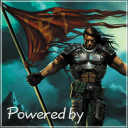
\includegraphics[width=.15\textwidth]{powered}
\item\label{item:morestats} More Statistics: The SmartCTF interface registers a lot more CTF game relevant events and generates the ``appropriate'' rewards (which can be configured in {\color{Purple}SmartCTF.ini}).  This list includes
  \begin{itemize}
  \item Covers: Rewards score and adrenaline\footnote{The methodology is written in Section \ref{Sec:coverseal}.}
  \item Seals: Rewards score and adrenaline.  
  \item FlagKills
  \item Captures
  \item (Flag) Grabs
  \item {\color{Red}First Blood}
  \item Frags
  \item Efficiency: Defined by the equation
    \begin{equation}
      \text{Eff} = \frac{\text{Frags}}{\text{Frags} + \text{Deaths}}
    \end{equation}
  \item Points
  \item Amps
  \item Suicides
  \item HeadShots 
\item \parbox[b]{.7\textwidth}{\item Nation: The CountryFlag  
\includegraphics[width=.05\textwidth]{Is}}
  \end{itemize}
\item More MultiPlayer, Team and Server information
  \begin{itemize}
  \item Average/individual pings, packetlosses and netspeeds are computed and shown.
  \item The Server TickRate is displayed in the Title component.  For more information on TickRates visit \href{http://wiki.unrealadmin.org/Netspeed_Tutorial_(UT)}{\color{Blue}Netspeed Tutorial}.
  \item Current Date (Day-Month-Year)/Time and Elapsed Time are obtained and shown in the Title component of ScoreBoard.
  \item The Server name and Map name are shown in the Scoreboard.
  \end{itemize}
\item Messaging System: SmartCTF has a unique way of broadcasting the Cover/Seal message to all the players.  The hope is to encourage players more for Covering the FlagCarrier or Sealing the Base over the ``Narcissist'' DeathMatch gameplay mentality.  Furthermore, SmarCTF can broadcast global messages related to ``MonsterKill'' and above.
  \item Scoreboard: The most admirable component of SmartCTF\SmartVersion~is the Scoreboard (Figure \ref{fig:smartscoreboard}).  It consists of the title and the body.  The title of the Scoreboard is divided in two components
    \begin{itemize}
    \item Header: shows the current state of the game.
    \item Footer: shows the spectator list (with Epic's bugfix!), current date/time and elapsed time
    and server/map name with the ``Tickrate''.
    \end{itemize}
The body of the scoreboards shows more player statistics.
\item Statistics Restoration: SmartCTF\SmartVersion~ has the capability to restore the statistics of the player who disconnected due to unfavorable circumstances (poor net connection, power fluctuations etc).  The resoration is done on the name basis. Total score can also be restored by setting bRecoverTotalScore to true as mentioned in section \ref{subsec:smartctf}.
\item Flag Carrier Location: SmartCTF can render the current location of the Flag Carrier at the top of the screen (below the team scores).
  \begin{figure}
\centering
\label{fig:fcloc}
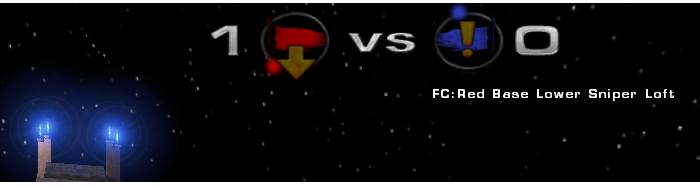
\includegraphics[width=0.8\textwidth]{fcloc}
\caption{A screenshot of FC location.}
\end{figure}
  
\end{itemize}

\section{Working}
In this section, we will explore the actual but brief working of SmartCTF by directly referencing the ``UnrealScript Code''.  Once we understand the code, we can perform further tweaks to enhance the gameplay.

\subsection{Witness}
\label{Sec:witness}
The class {\color{Orange}SmartCTF.uc} spawns an instance named ``Witness'' to enforce actual counting of the player statistics.  The code is 
\begin{lstlisting}[frame=single]
     Witness = Level.Game.Spawn(class'UTServerAdminSpectator');
     if(Witness != none){
        Log("| Successfully Spawned the Witness"@Witness, 'SmartCTF');
        Witness.PlayerReplicationInfo.PlayerName = "Witness";
     }
     else
        Log("ERROR! Couldn't Spawn the Witness", 'SmartCTF');
%* \ldots *)
\end{lstlisting}

The role of the ``Witness'' is to silently spectate the game and receive the game messages.  Then in the function ``EvaluateMessageEvent'', as follows,

\begin{lstlisting}[frame=single]
  switch(Switch){
          // CAPTURE
          // Sender: CTFGame, PRI: Scorer.PlayerReplicationInfo, OptObj: TheFlag.Team
          case 0:
             if(MessagingSpectator(Receiver) == Witness){
                ReceiverStats = SCTFGame.GetStats(Controller(RelatedPRI_1.Owner));
                if(ReceiverStats != none) ReceiverStats.Captures++;
                ResetSprees(0);
                ResetSprees(1);
                FCs[0] = none;
                FCs[1] = none;
             }
             break;
%* \ldots *) 
\end{lstlisting}
line 5 essentially makes sure that line 7 gets executed only once.  Otherwise the ``Capture'' counter will increase the number of times the function ``EvlauateMessageEvent'' is executed which is equal to the number of Human players in the game.

Note that the ``Witness'' is never shown in the spectator list of the ``SmartScoreboard''.  This can be easily seen from the line 9 of the code (in {\color{Orange}SmartCTFScoreBoard.uc})

\begin{lstlisting}[frame=single]
  function string GetSpectatorString(){

    local string ReturnString;
    local int i;

    if(GRI == none || !GRI.bMatchHasBegun)// No spectators are shown during the Match Survey
       return "";
    for(i = 0; i < GRI.PRIArray.Length; i++){
       if(GRI.PRIArray[i].bIsSpectator && GRI.PRIArray[i].PlayerName != "Witness"){
          if(ReturnString == "")
             ReturnString = ReturnString@GRI.PRIArray[i].PlayerName;
          else
             ReturnString = ReturnString$","@GRI.PRIArray[i].PlayerName;
       }
    }
    return ReturnString;
 }
\end{lstlisting}

\subsection{Covers/Seals}
\label{Sec:coverseal}
Consider the situation in which Red players PlayerR1 and PlayerR2 (with the Blue flag) and Blue player PlayerB1 (with or without Red flag) are involved.  PlayerR1 kills PlayerB1.  In code\footnote{The code written in this section can be located in {\color{Orange}SmartCTF.uc}}:

\begin{lstlisting}[frame=single]
  if(KillerPRI.HasFlag == none && FCs[KillerPRI.Team.TeamIndex] != none && FCs[KillerPRI.Team.TeamIndex].PlayerReplicationInfo.HasFlag != none)
\end{lstlisting}

We define ``Cover'' when: 
\begin{itemize}
\item PlayerB1 was killed within 576 uu (Unreal Units\footnote{These are the units for UT2004.  For more information on units, consult \href{https://wiki.beyondunreal.com/Unreal_Unit}{{\color{Blue}UnrealWiki}}.}) of PlayerR2
\item or PlayerR1 was within 576 uu of PlayerR2
\item or PlayerB1 could see PlayerR2 and was killed within 1728 uu of PlayerR2
\item or PlayerB1 had direct line-of-sight to PlayerR2 and was killed within 864 uu of PlayerR2.
\end{itemize}

Note that these figures are obtained from experience and are open for further modifications based on appropriate discussions!



Code is: 
\begin{lstlisting}[frame=single]  % Start your code-block

if((VSize(Killed.Location - FCs[KillerPRI.Team.TeamIndex].Pawn.Location) < 512*1.125)
       || (VSize(Killer.Pawn.Location - FCs[KillerPRI.Team.TeamIndex].Pawn.Location) < 512*1.125)
       || (VSize(Killed.Location - FCs[KillerPRI.Team.TeamIndex].Pawn.Location) < 1536*1.125 && Killed.Controller.CanSee(FCs[KillerPRI.Team.TeamIndex].Pawn))
       || (VSize(Killed.Location - FCs[KillerPRI.Team.TeamIndex].Pawn.Location) < 1024*1.125 && Killer.CanSee(FCs[KillerPRI.Team.TeamIndex].Pawn))
       || (VSize(Killed.Location - FCs[KillerPRI.Team.TeamIndex].Pawn.Location) < 768*1.125 && Killed.Controller.LineOfSightTo(FCs[KillerPRI.Team.TeamIndex].Pawn))){
       // Killer DEFENDED THE Flag CARRIER
          if(KillerStats != none){
             KillerStats.Covers++;
             KillerStats.CoverSpree++;// Increment Cover spree
             if(KillerStats.CoverSpree == 3){// Cover x 3
                BroadcastLocalizedMessage(class'SmartCTFMoreMessages', 2, KillerPRI);
             }
             else if(KillerStats.CoverSpree == 4){// Cover x 4
                BroadcastLocalizedMessage(class'SmartCTFMoreMessages', 1, KillerPRI);
             }
             else{// Cover
                BroadcastLocalizedMessage(class'SmartCTFMoreMessages', 0, KillerPRI);
             }
          }
          KillerPRI.Score += CoverReward;// Cover Bonus
          Killer.AwardAdrenaline(CoverAdrenalineUnits);
       }  
\end{lstlisting}
Lines 8 increases the Cover counter (which is displayed in the Scoreboard), lines 11, 13 and 17 broadcast the message to all the players on HUD and lines 20 and 21 provide the appropriate rewards to the player.

We define ``Seal'' when:
\begin{itemize}
\item PlayerR2 is in ``Red FlagZone''\footnote{For definition of FlagZone we refer the reader to Section .} and Red flag is \emph{not} with any Blue player.
\item PlayerB1 is killed in ``Red FlagZone''.
\end{itemize}

The relevant code is
\begin{lstlisting}[frame=single]
  bKilledTeamHasFlag = true;
       if(FCs[KilledPRI.Team.TeamIndex] == none) bKilledTeamHasFlag = false;
       if(FCs[KilledPRI.Team.TeamIndex] != none &&
        FCs[KilledPRI.Team.TeamIndex].PlayerReplicationInfo.HasFlag == none) bKilledTeamHasFlag = false;// Safety check

       // if Killed's FC has not been set / if Killed's FC doesn't have our Flag
       if(!bKilledTeamHasFlag){
          // If Killed and Killer's FC are in Killer's Flag Zone
          if(IsInZone(KilledPRI, KillerPRI.Team.TeamIndex) && IsInzone(FCs[KillerPRI.Team.TeamIndex].PlayerReplicationInfo, KillerPRI.Team.TeamIndex)){
             // Killer SEALED THE BASE
             if(KillerStats != none)
                KillerStats.Seals++;
             BroadcastLocalizedMessage(class'SmartCTFMoreMessages', 3, KillerPRI);
             KillerPRI.Score += SealAward;//Seal Bonus
             Killer.AwardAdrenaline(SealAdrenalineUnits);
          }
       }
\end{lstlisting}

\subsection{Replication}
Replication is one of the very important aspects of Unreal Engine.  So important that Tim Sweeney\footnote{If you don't know him, you should probably purge this document.} wrote an article exclusively for it in 1999-07-21 (for the current avatar of the document visit \href{https://api.unrealengine.com/udk/Three/NetworkingOverview.html}{{\color{Blue}Unreal Networking Architecture}}).  In this section I will demonstrate the ``Replication at Work'' from ``Live Example''.  One of the central features of SmartCTF is to collect and display lot more statistics (see Section \ref{sec:features}).  These statistics are generated on the server instance of the game.  On the other hand statistics are displayed on the client instance of the game connected to server via internet or LAN (party?).

First we spawn an {\color{Cyan}Actor} named ``SmartCTFPlayerReplicationInfo'' which inherites is properties from the base class ``ReplicationInfo''.  This is done by the code (in {\color{Orange}SmartCTF.uc})
\begin{lstlisting}[frame=single]
  function AssociateSmartReplication(Pawn Other){

       local SmartCTFPlayerReplicationInfo NewSPRI;
       local int i;

       NewSPRI = Spawn(class'SmartCTFPlayerReplicationInfo', Other.PlayerReplicationInfo);
       NewSPRI.SPlayerName = Other.PlayerReplicationInfo.PlayerName;
       NewSPRI.SPlayerID = Other.PlayerReplicationInfo.PlayerID;
       NewSPRI.IpToNation = IpToNation;
       NewSPRI.bIpToNation = true;
       for(i = 0; i < GoneSmartPRI.Length; i++){
          if(GoneSmartPRI[i] != none && Other.PlayerReplicationInfo.PlayerName == GoneSmartPRI[i].SPlayerName){// Include IP check?
             NewSPRI.CopyStats(GoneSmartPRI[i]);
             GoneSmartPRI.Remove(i, 1);// Save the bandwidth :D
          }
       }
 }
%* \ldots *) 
\end{lstlisting}
This code is executed on both server and client machines.  Line 6 essentially spawns the {\color{Cyan}Actor} on both the machines and sets the ``Owner'' of this instance as {\color{Cyan}PlayerReplicationInfo} (which itself is an {\color{Cyan}Actor}).  But the owner is \emph{not} set client side.  Therfore we need a way to identify this instance from client side (for example while displaying the ScoreBoard).  We can do this by assigning a unique ``number'' to a memberdata of the instance. Fortunately this number is generated by the engine and known as {\color{Magenta}PlayerID} memberdata of class ``PlayerReplicationInfo''. 

The server instance always has the bleeding (updated) values of all the  memberdata.  Thus from line 8 we assign the ID to the {\color{Cyan}Actor} instance of class ``SmartCTFPlayerReplicationInfo''.  But this is done serverside.  The client (as usual) is sitting dumb ignorant of this information.  So in order to make sure that the information ``flows'', we replicate the memberdata in the ``SmartCTFPlayerReplicationInfo'' by using the code

\begin{lstlisting}[frame=single]
  replication{
%* \ldots *) 
    // Things the server should send to the client.
	reliable if (bNetDirty && (Role == Role_Authority))
		NetSpeed, NationPrefix, SPlayerName, SPlayerID;
%* \ldots *) 
 }
\end{lstlisting}
Now any function, executed from client instance can easily access the memberdata {\color{Magenta}SPlayerID}.  The example can be easily seen by the code
\begin{lstlisting}[frame=single]
 simulated function SmartCTFPlayerReplicationInfo GetStats(PlayerReplicationInfo A){

  local int i;

  if(A == none) return none;
  ReloadBuffer();// Collect the swarm of SmartCTFPlayerReplication instances.
  for(i = 0; i < PRIBuffer.Length; i++){
     if(A.PlayerID == PRIBuffer[i].SPlayerID){
        return PRIBuffer[i];
     }
  }
  return none;
 }
\end{lstlisting}
Here, when the code is being executed on the client instance, line 8 is useful only if {\color{Magenta}SPlayerID} has already replicated properly to the client.

\subsection{SmartScoreboard}
\label{sec:smartscoreboard}
I have taken the help of Epic's default Scoreboard for the ``Compression Scheme'' and SmartCTF's years of experience in setting the layout.  The end result is that it can show the statistics of 23 players with the resolution of $1680 \times 1050$ without cluttering the screen.  Most of the code is self explanatory (see the associated comments to get a deep understanding).  However there are few code snippets that require explainnation.

First, the scoreboard is drawn on the abstract instance {\color{Purple}Canvas}.  In order to work with the instance, there is a natural sequence of code is written

\begin{lstlisting}[frame=single]
  Canvas.Font = SomeFont;// Sets the Font Size
  Canvas.Strlen("Test", XL, YL);
  Canvas.SetPos(SomeX, SomeY);// Sets the Position on the Screen
  Canvas.DrawColor = SomeColor;// Sets the Color
  Canvas.SomeDrawCommand(Some Arguments);// Actual Draw Command
\end{lstlisting}

Line 2 essentially measures the width and height of the text 'Test' with the ``said'' fontsize.  It is useful to estimate the position of ``next'' possible drawing item.

\subsubsection{Compression Scheme}
The  compression of the scoreboard is done by reducing the fontsize of the text ``PlayerName'' in 4 stages.  The rest of the structural components which include ``PlayerBoxSizeY'' (the height of individual PlayerBox) and ``BoxSizeY'' (the height of header box) are computed accordingly.

The code is 
\begin{lstlisting}[frame=single]
  if(MaxPlayerCount > (C.ClipY - MessageFoot)/(PlayerBoxSizeY + BoxSpaceY)){
	   // Compress the Scoreboard: Decrease the Header Box
	   BoxSpaceY = 0.125 * YL;
	   if(MaxPlayerCount > (C.ClipY - MessageFoot)/(PlayerBoxSizeY + BoxSpaceY)){
	      // Compress the Scoreboard: Decrease individual PlayerBoxSize and Font
	      FontReduction++;
	      C.Font = GetSmallerFontFor(C, FontReduction);
	      C.StrLen("Test", XL, YL);
	      BoxSpaceY = 0.125 * YL;
	      if (HaveHalfFont(C, FontReduction))
	         PlayerBoxSizeY = 2.125 * YL;
	      else
	         PlayerBoxSizeY = 1.75 * YL;
	      HeadFoot = 4*YL + IconSize;
          if(MaxPlayerCount > (C.ClipY - MessageFoot)/(PlayerBoxSizeY + BoxSpaceY)){
             // Compress further by reducing Font
             FontReduction++;
             C.Font = GetSmallerFontFor(C, FontReduction);
	         C.StrLen("Test", XL, YL);
	         BoxSpaceY = 0.125 * YL;
	         if (HaveHalfFont(C, FontReduction))
	            PlayerBoxSizeY = 2.125 * YL;
	         else
	            PlayerBoxSizeY = 1.75 * YL;
	         HeadFoot = 4*YL + IconSize;
	         if(C.ClipY >= 600 && (MaxPlayerCount > (C.ClipY - HeadFoot)/(PlayerBoxSizeY + BoxSpaceY))){
	            // Compress further if Resolution is High enough (Why HeadFoot?)
	            FontReduction++;
                C.Font = GetSmallerFontFor(C, FontReduction);
	            C.StrLen("Test", XL, YL);
	            BoxSpaceY = 0.125 * YL;
	            if (HaveHalfFont(C, FontReduction))
	               PlayerBoxSizeY = 2.125 * YL;
	            else
	               PlayerBoxSizeY = 1.75 * YL;
	            HeadFoot = 4*YL + IconSize;
	            if(MaxPlayerCount > (C.ClipY - 1.5 * HeadFoot)/(PlayerBoxSizeY + BoxSpaceY)){
                   // final Compression
                   FontReduction++;
                   C.Font = GetSmallerFontFor(C, FontReduction);
	               C.StrLen("Test", XL, YL);
	               BoxSpaceY = 0.125 * YL;
	               if (HaveHalfFont(C, FontReduction))
	                  PlayerBoxSizeY = 2.125 * YL;
	               else
	                  PlayerBoxSizeY = 1.75 * YL;
	               HeadFoot = 4*YL + IconSize;
                }
             }
          }
       }
    }
\end{lstlisting}

\section{Developing}
SmartCTF is open-source project with the online repository on \href{https://github.com/ravimohan1991/SmartCTF}{{\color{Blue}GitHub}}.  You are welcome to fork the repository and produce modifications/improvements.
\subsection{ScoreBoard}
The most appropriate layout of the ``SmartScoreboard'' is already set.  What is required is an appropriate ``Color Scheme''.  It means applying appropriate colors to various components of the the scoreboard in the most visually appealing manner.  In order to apply the scheme, one can first consult the code of section \ref{sec:smartscoreboard}.

UT99 community has developed a snowy version of the scoreboard with ``animated'' snow falling down.  Similar techniques can be applied to the ``SmartScoreboard'' to render the snow!

\begin{figure}
\centering
\label{fig:snowyscoreboard}
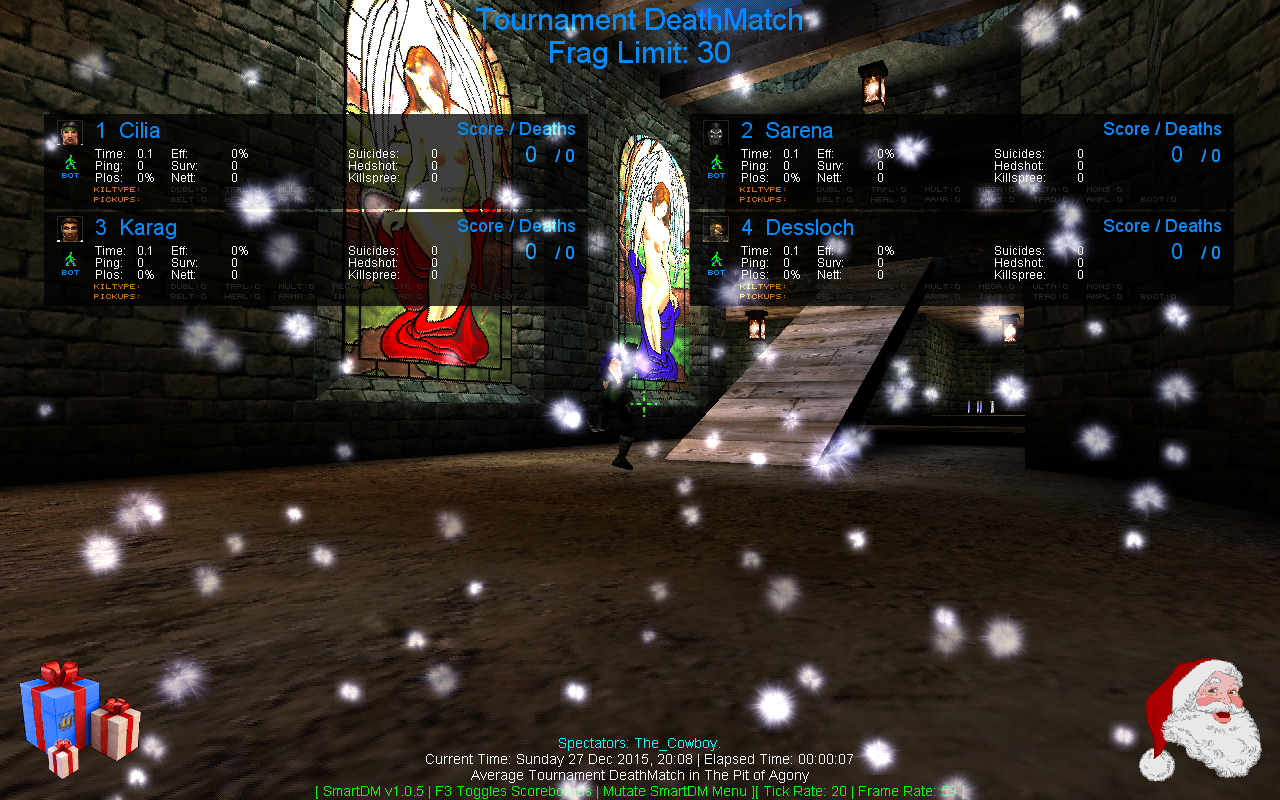
\includegraphics[width=1.1\textwidth]{snowy}
\caption{A screenshot of the snowy scoreboard.}
\end{figure}


\section{TODO}
As far as coding is concerned, I have done most of it.  One feature might be adding the ``SpawnKill'' detection.  I leave it for the future.
Now it would be cool to add various resources to SmartCTF.  The list includes
\begin{itemize}
\item Announcer Sounds for the ``Cover'' and ``Seal''.  And I am talking about the good ol' Classic Announcer-style!
\item Textures for the Scoreboard including background, FirstBlood, and partition generators.  Animated textures would be cool.  {[es]}Rush has already done awesome job with the CountryFlags textures.  It would be nice to have better textures for FC in the socreboard (Figure \ref{fig:smartscoreboard}).
\end{itemize}

\section{ChangeLog}
\begin{changelog}[author=The\_Cowboy,
                  sectioncmd=\subsection,
                  title=SmartCTF changelog]
\begin{version}[v=1C(Unreleased)]
\fixed
     \item bDisableOvertime not ending the game time.
     \item Map radar image showing in some maps (for example see \href{https://github.com/ravimohan1991/SmartCTF/issues/4}{\color{blue}here}).
\added
     \item bShowCountryFlags
     \item bShowFirstBlood
     \item bRecoverTotalScore
\deprecated
     \item All the SmartCTF settings are now stored in {\color{Purple}UT2004.ini} or {\color{Purple}Server.ini} as per the \href{https://github.com/ravimohan1991/SmartCTF/issues/3}{{\color{Blue}request}}. 
\end{version}
\begin{version}[v=1B, date=2020-06-10]
\added
     \item bDisableOvertime
\fixed
     \item Statistics replication for players leaving server.
\end{version}
\shortversion{v=1A, date=2019-04-16, changes=Initial release.}  
\end{changelog}


\section{Credits}
SmartCTF has a rich and animated histroy due to the contributions of several outstanding coders and their inspirations.  The list (in no particular order) includes
\begin{itemize}
\item \{PiN\}Kev
\item \{DnF2\}SiNiSTeR
\item {[es]}Rush
\item Adminthis
\item Sp0ngeb0b 
\end{itemize}

For this UT2k4 port, I would like to especially thank
\begin{itemize}
\item Wormbo (for his ServerLogo mod and endless contribution in the programming universe of Unreal Engine)
\item \href{https://github.com/Annihilator}{\color{Blue}Annihilator} for mutator testing and constructive feedback.
\item {[es]}Rush and Matthew 'MSuLL' Sullivan for IpToCountry methods
\item Epic Games for releasing new versions of the ``Game we Love''
\end{itemize}

Finally the online resources
\begin{itemize}
\item \href{https://ut-files.com/}{{\color{Blue}https://ut-files.com/}}
\item \href{http://unrealtournament.99.free.fr/}{{\color{Blue}http://unrealtournament.99.free.fr/}}
\end{itemize}
A big thanks for keeping the ``ancient goodwill'' intact!
\end{document}